\section{Stromrichterschaltung}
\subsection{Gruppierung}
\subsubsection{nach Steuerung}
\begin{itemize}
    \item Ungesteuerte Stromrichter:
        \subitem Das Verhältniss von Eingans- zu Ausgangsspannung wird durch die Stromrichterschaltung festzgesetzt
    \item Gesteuerte Stromrichter
        \subitem Das Verhältniss von Eingans- zu Ausgangsspannung wird durch Steuereingriff am Halbleiterschalter verändert. 
\end{itemize}

\subsubsection{nach Führung}

\href{https://de.wikipedia.org/wiki/Kommutierung}{Kommuntierung WIKI}\newline
Bzw nach der Herlkunft der Kommutierungssoannung.\newline
Kommutierung bedeutet die Wechslung des Stromflusses con einem HL-Ventil auf ein anderes.
\begin{itemize}
    \item Netzgeführte Schaltung
        \subitem Kommutierungsspannung vom Netzwerk
    \item Lastgeführte Schaltung
        \subitem Kommuntierungsspannung wird durch Lastkreis (zb Synchronmotor) gesteuert
    \item Selbstgeführte Schalung
        \subitem Kommutierungsspannung wird selbst erzeugt
\end{itemize}

\subsection{Kennzeichnung}
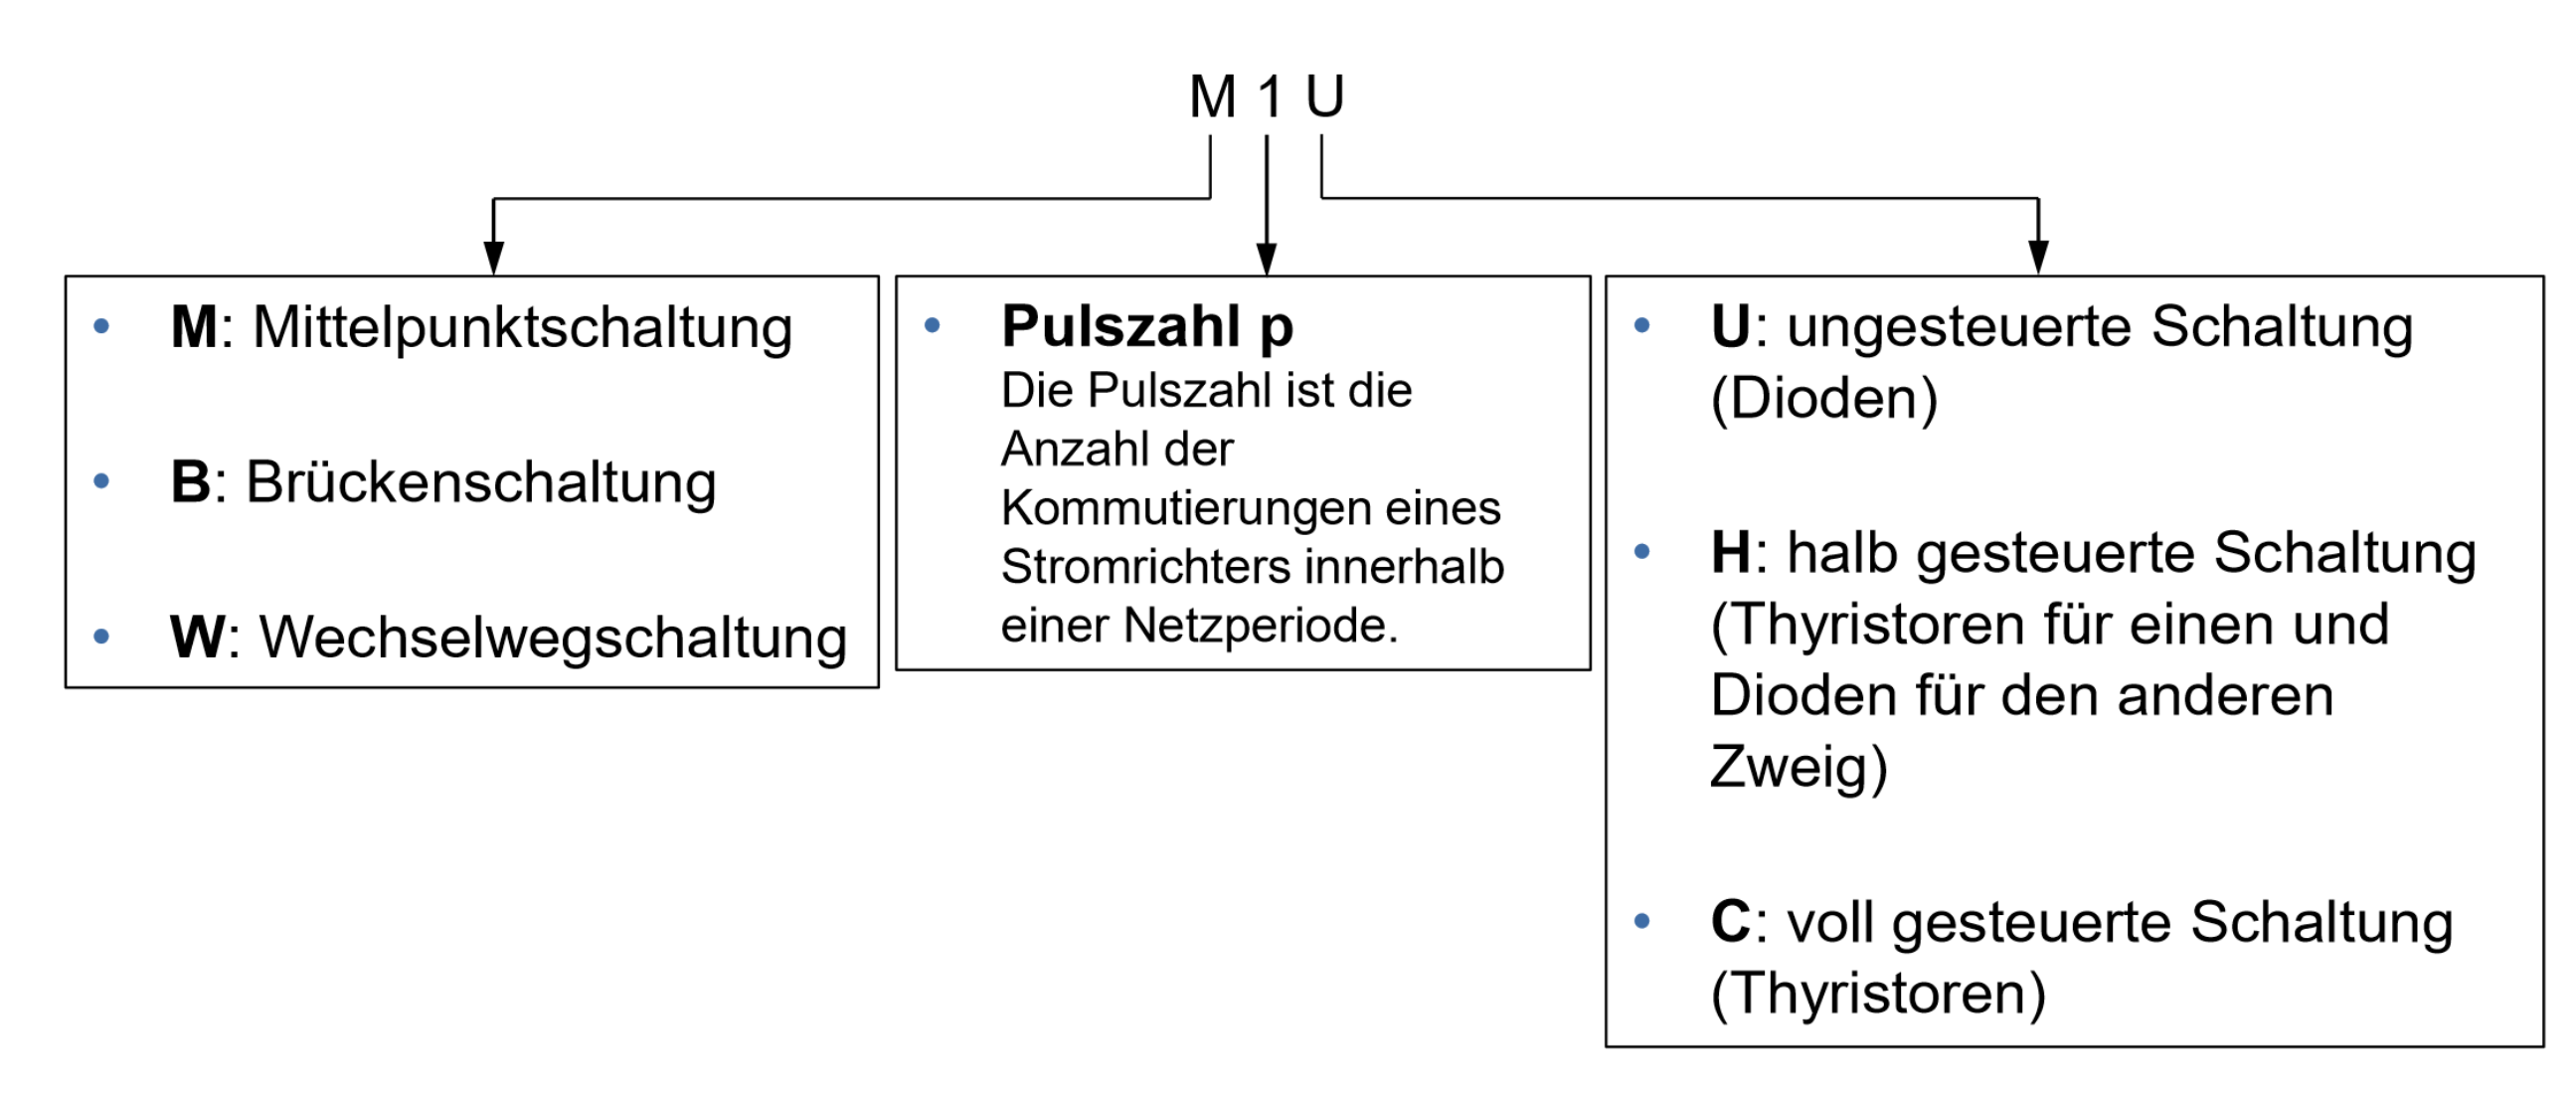
\includegraphics[width=0.8\linewidth]{images/SRKennzeichnung}\newline
\href{https://de.wikipedia.org/wiki/Gleichrichter}{Gleichrichter WIKI}

\subsection{Ungesteierter Gleichrichter (M1U)}
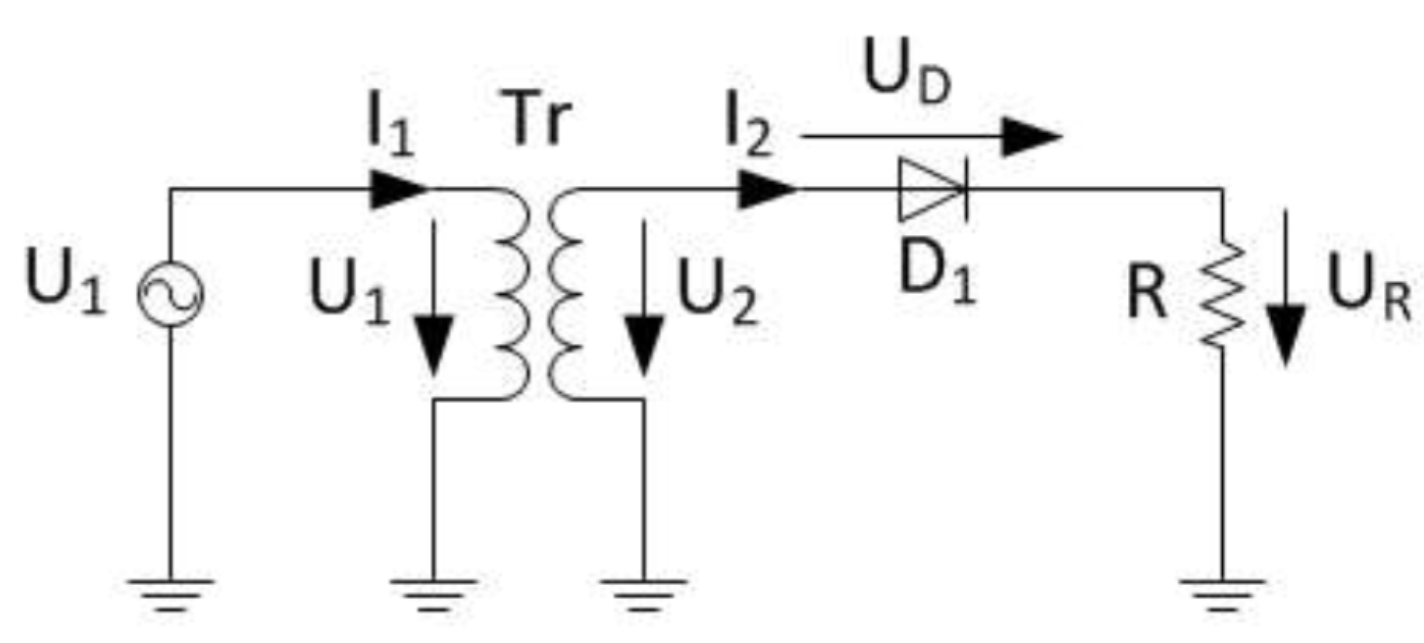
\includegraphics[width=0.4\linewidth]{images/UGRM1U}
Die Diode wird als Ideal betrachtet \rightarrow keine Schwellenspannung oder Innenwiderstand

\begin{longtable}{| p{.25\textwidth} | p{.40\textwidth} | p{.30\textwidth} |} %TODO Formeln einfügen
    \hline
    \textbf{Grundgleichungen}&
    \[ U_2 = U_D + U_R \]
    \[ U_R = I_2 \cdot R \]&\\
    \hline
    \textbf{Durchlassrichtung}\newline
    $ 0 < \omega t < \pi $&
    \[ U_2 = U_R \qquad U_D = 0 \]&\\
    \hline   
    \textbf{Sperrichtung}\newline
    $ \pi < \omega t < 2\pi $&
    \[ U_2=U_D \qquad U_R = 0 \]&\\
    \hline
    
    &
    &
    \\ \hline
    
    \textbf{Scheinleistung}&
    \[ S_2 = U_2 \cdot I_2 = U_2 \cdot I_{R RMS} \]&
    \\ \hline
        
    \textbf{Grundschwingugngsblindleistujng}&
    \[ Q_2\cdot I_{2 1} \cdot sin(\varphi_{2 1}) = 0 \]&
    \\ \hline    
    
        
    \textbf{Verzerrungsleistubg}&
    \[ Q_v = U_2 \cdot \sqrt{\sum_{k=2}^{\infty} {I_2^2}_k} = \sqrt{S_2^2 - P_2^2} \]&
    \\ \hline

\end{longtable}
%
%Leistung = Momentanleistung des Sormes x momentanleistung der Spannung\\
%Leistung = Leistung bei trafoseite messen 1harm des stroms phasenverschiebung -> u i cos(phi) fourierreihen..
%Leistung = Irav* U1harm  

\subsection{Ungesteuerter Gleichrichter (B2U)}


\clearpage